\documentclass[12pt]{report}

\usepackage{amsmath, amsfonts}
\usepackage{eucal}
\usepackage{graphicx}
\usepackage{enumitem}
\usepackage{tikz}

\newtheorem{definition}{Definition}
\newtheorem{example}{Example}

\newcommand{\bfit}[1]{\textbf{\textit{#1}}}


\title{\textbf{Engineering Mathematics}}
\author{\textbf{F17/2054/2022} - ROBERT ODHIAMBO}
\date{November 5, 2023}
\begin{document}

\maketitle

\chapter*{Basic mathematical Concepts}

    \section*{Sets}
        \begin{definition}
            A set is a well defined collection or group of objects.
        \end{definition}
        \text{These objects are also referred to as members of a set}
        \begin{enumerate}
            \item Requirements of a set \\
                \begin{enumerate}
                    \item A set must be well defined, i.e, must not leave room for any ambiguity.
                    \item The elements of a given set must be distinct, i.e,\\
                    \text{each element should appear only once.}
                    \item The order of representing elements of a set is immaterial,\\
                    \text{different arrangement of the
                    same elements does not showany difference.}
                \end{enumerate}
            \item Specifying or naming of sets \\
                \text{By convention, sets are specified (named) using a capital letter.}\\ 
                \text{Further, the elements of a set are designated by either listing all}\\ 
                \text{the elements or by using a descriptive characteristic or pattern. The} \\
                \text{elements of a set are enclosed using curly brackets. We can represent them in three ways:} \\
                \begin{itemize}
                    \item[$-$] Listing of all elements \\
                    $ A = \{0,1,2,3,4,5,6\}$
                    \item[$-$] Using a descriptive characteristic \\
                    $ A = \{\textit{A such that X is a positive integer from 0 to 6 inclusive} \} $
                    \item[$-$] Using a pattern \\
                    $ A = \{1,2,\ldots,6\}$
                \end{itemize}
            \item Set membership \\
                \text{This is  expressed by using the symbol $\in$. Considering set}\\
                \text{\textit{A} in which 3 is a member}
                \text{Expressed as 3 \(\in\) \textit{A}}
            \item Finite set \\
                \text{A set that consists of a limited or countable number of elements.}
            \item Subset \\
                \text{Any set \textit{S} is a subset of set \textit{A} if all elements in}\\
                \text{\textit{S} are members of \textit{A} and is denoted} \\
                \text{by $\subset$ and is read as "\textit{S} is a subset of \textit{A}"} \\
                \text{A is said to be the superset of S denoted by $\supset$, $A \supset S$}
            \item Equality of Sets \\
                \text{If all elements in set D1 are in D2 and all the elements in D2 are}\\
                text{in D1 then they are equal D1 = D2}\\
                \text{Can be denoted as $D1 \supset D2 \text{or} D2 \subset D1$, i.e,}\\
                text{they are subsets or supersets of each other.}
            \item Universal Set \\
                \text{Set that contains all the elemnts under consideration,denoted U.}
            \item Null or empty set \\
                \text{Is a set with no elements and is denoted by \{\} or $\emptyset$.}
            \item Complement of a set \\
                \text{Given U and $A \subset U$ then the complement of A, denoted by A'}\\
                \text{or $A^c$ represents all elements} \\
                \text{in U that are not in A.}
            \item Seys are pictorially represented using Venn Diagrams \\
                \text{ }\\
                \textbf{Symbols} \\
                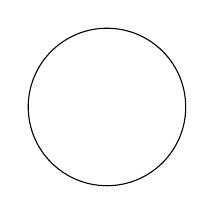
\begin{tikzpicture}
                    \draw (0,0) circle(10mm);
                \end{tikzpicture} \\
                \text{ }\\
                \text{Circles: used to represent ordinary sets}\\
                \text{ }\\
                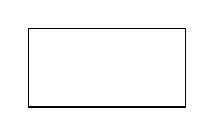
\begin{tikzpicture}
                    \draw (0,0) -- (2,0) -- (2,1) -- (0,1) --cycle;
                \end{tikzpicture}\\
                \text{ }\\
                \text{Rectangle: Used to represent Universal set}\\
            \item Singleton Set \\
                \text{Set with only one element}
            \item Disjoint sets \\
                \text{Are two sets with no elements in common}
        \end{enumerate}

    \section*{Set Operations and Algebra}
        \begin{definition}
            \text{These are operations where sets are combined to obtain other sets of interest}
        \end{definition}

        \text{Given two sets P and Q}\\

        \text{They include:}\\
        \begin{enumerate}
            \item \textbf{Union of Sets, $\cup$} \\
                \text{Consists of elements in P or Q or both}
                \begin{figure}[h!]
                    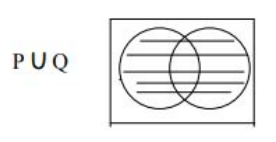
\includegraphics[width=0.4\linewidth]{union.png}
                \end{figure}
            \item \textbf{Intersection of sets, $\cap$} \\
                \text{Consists of elements in both P and Q(common elements)}
                \begin{figure}[h!]
                    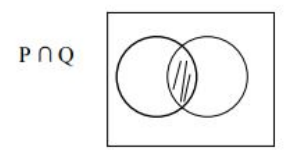
\includegraphics[width=0.4\linewidth]{intersection.png}
                \end{figure}
            \item \textbf{Set difference/Injunction, $\setminus$} \\
                \text{Consists of elements in P but not in Q}
                \begin{figure}[h!]
                    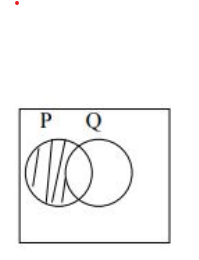
\includegraphics[width=0.4\linewidth]{set_difference.png}
                \end{figure}
            \item \textbf{Symetric difference, $\Delta$} \\
                \text{Consists of elements in P but not in Q and thos in Q but not in P}
                    \begin{figure}[h!]
                        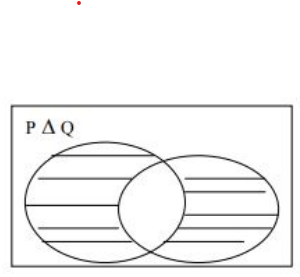
\includegraphics[width=0.4\linewidth]{symmetric_diff.png}
                    \end{figure}
        \end{enumerate}

    \section*{Laws of Set aAlgebra}
        \begin{enumerate}
            \item Commutative Laws \\
                \text{The order in which sets are combined in union or intersection is irrelevant, i.e}
                \text{$P \cup Q = Q \cup P$ and $P \cap Q = Q \cap P$}
            \item Associative Laws \\
                \text{The selection of 3 or more sets for grouping in a union or intersection}\\
                \text{is immaterial, i.e}
            $(P \cup Q) \cup R = P \cup (Q \cup R)$
            \item Distributive Laws \\
                \text{For any 3 sets P, Q and R:}\\
            $P \cup (Q \cap R) = (P \cap Q) \cap (P \cup R)$        
            \item Impotent Laws \\
                \text{For a set Q}\\
                $Q \cup Q = Q$ \text{and} $Q \cap Q = Q$\\
                \textbf{Other Laws: } \\
            \item $P \cup \emptyset = P$ \\
            \item $P \cap \emptyset = \emptyset$ \\
            \item $P \cup U = U$ \\
            \item $P \cap U = P$ \\
            \item $P \cup P' = U$\\
            \item $P \cap P = \emptyset$\\
            \item De Morgan's Laws\\
                \text{For  any two sets Q and R}\\
                \begin{itemize}
                    \item[i] $(Q \cup R)' = Q' \cap R'$
                    \item[ii] $(Q \cap R)' = Q' \cap R'$
                \end{itemize}
        \end{enumerate}
    \section*{Boolean Algebra}
        \text{Can be used to describe the manipulation and processing of binary information}\\
        \text{It's two-valued and has applications in the design of modern computer systems.}\\
        \text{It is common to inteprete the digital values 0 as false and 1 as true.}\\
        \text{ }\\

        \textbf{Definitions} \\
        \begin{enumerate}
            \item Boolean Expression: Combining the variables and operation yields Boolean
            expressions.
            \item Boolean Function: A Boolean function typically has one or more input
            values and yields a result, based on these input value, in the range 0, 1.
            \item A Boolean operator can be completely described using a table that list
            inputs, all possible values for these inputs, and the resulting values of
            the operation.
            \item A truth table shows the relationship, in tabular form, between the input
            values and the result of a specific Boolean operator or function on the
            input variables.
                \begin{figure}[h!]
                    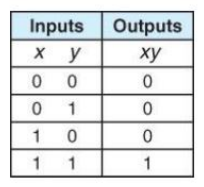
\includegraphics[width=0.3\linewidth]{AND_tt.png}
                    \caption{Truth table for AND}
                \end{figure}
            \item The AND operator is also known as a Boolean product. The Boolean
            expression xy is equivalent to the expression x * y and is read “x and y.”
            The behavior of this operator is characterized by the truth table shown
            below
                \begin{figure}[h!]
                    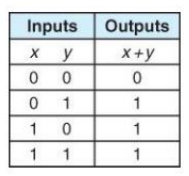
\includegraphics[width=0.3\linewidth]{OR_tt.png}
                    \caption{Truth Table for OR}
                \end{figure}
                \begin{figure}[h!]
                    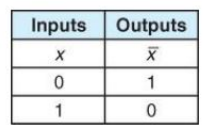
\includegraphics[width=0.3\linewidth]{NOT_tt.png}
                    \caption{Truth table for NOT}
                \end{figure}
            \item The OR operator is often referred to as a Boolean sum. The expression
            x+y is read “x or y”. The truth table for OR is shown below
            \item Both $\bar{x}$ and $x'$ are read as NOT x 
            \item The rule of precedence for Boolean operators give NOT top priority,
            followed by AND, and then OR
        \end{enumerate}

        \text{\textbf{DeMorgan's law} provides an easy way of finding the complement of a Boolean function.}\\
        \text{Boolean algebra is used in implementing digita computer circuits called \textbf{gates}.}

        \begin{figure}[h!]
            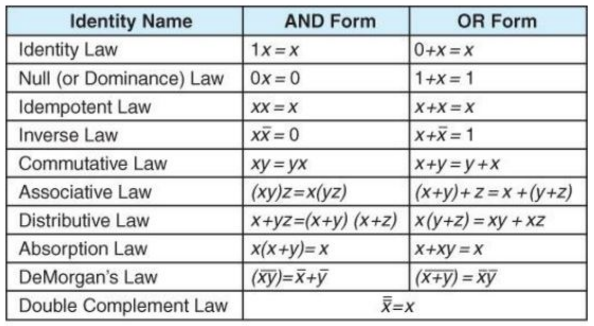
\includegraphics[width=\linewidth]{basic_identities.png}
            \caption{Basic Identities of Boolean Algebra}
        \end{figure}
        

\chapter*{Cartesian Products and Relations}

    \text{For two sets \textit{A} and $B$, the Cartesian Product of \textit{A} and $B$ is\\}
    $$A \times B = \{(a, b); a \in A, b \in B\}$$
    \text{We say that the elements of \textit{A} \(\times\) $B$ are ordered pairs\\}

    \begin{definition}
    : For sets A, B, any subset of \textit{A} \(\times\) $B$ is called a binary relation from
    \textit{A} to $B$. Any subset of \textit{A} \(\times\) \textit{A} is called a \textbf{binary relation} on \textit{A}.
    \end{definition}
    \text{A binary relation  from A to B is a set $\mathcal{R}$ of ordered pairs where the first element of each}\\
    \text{ordered pair comes from A and the second element comes from B. We use the notation $a\mathcal{R}b$ to}\\
    \text{denote that $(a,b) \in \mathcal{R} \text{ and a} \not \mathcal{R} b$ When $(a,b) \in \mathcal{R}, a$ is said to be related to $b \text{ by } \mathcal{R}$.}\\
    \text{Let $A=\{0,1,2\}$ and \(B=\{a,b\}\) then \(\mathcal{R}=\{(0,a),(0,b),(1,a),(2,b)\}\) is a relation from \textit{A} to \textit{B}.}\\
    \text{This means for instance that \(0\mathcal{R}a, 1\mathcal{R}a,\)etc}\\
    \text{The above relation can be represented graphically using arrows to represent ordered pairs: }
    \begin{figure}[h!]
        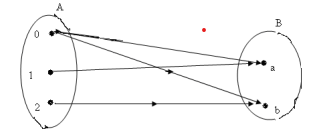
\includegraphics[width=0.4\linewidth]{relationns1.png}
        \caption{Graph for the relation explained above}
    \end{figure}

    \section*{Relations on a set}

        \begin{definition}
            A relation on a set A is a relation from A to A
        \end{definition}

        \begin{example}
            Let A=\{1,2,3,4\}. Which ordered pairs in the relation $\mathcal{R}=\{(a,b):a\text{ divide } b$\}\\
            \label{fig1}
        \end{example}

        \textbf{Solution}
        \text{Since \((a,b)\) is in $\mathcal{R}$ if and only if a and b are positive integers not exceeding 4 such}\\
        \text{that a divides b,wesee that:}\\
        $\mathcal{R=\{\text{(1,1), (1,2), (1,3), (1,4), (2,2), (2,4), (3,3), (4,4)}\}}$

        \begin{figure}[h!]
            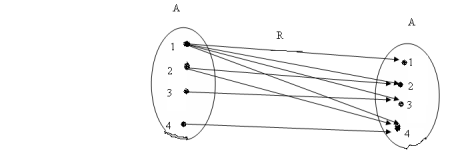
\includegraphics[width=0.5\linewidth]{relations2.png}
            \caption{Graph of the relation in example \ref{fig1}}
        \end{figure}

        \text{On a set \textit{A} with \textit{n} elements, a relation on \textit{A} is a subset of $A \times A$. Since $A \times A$ has $n^2$}\\
        \text{elements, when \textit{A} has \textit{n} elements and a set with \textit{m} elements has $2^m$ subsets, there are ${2^n}^2$}\\
        \text{subsets of $A \times A$. Thus there are \bfit{$2n^2$} relations on a set with \textit{n} elements.}

    \section*{Properties of Relations}

        \begin{definition}
            A relation $\mathcal{R}$ on a set A is said to be \bfit{reflexive} if for all $x \in A, (x,x) \in \mathcal{R}$.
        \end{definition}

        \begin{example}
            For A = \{1,2,3,4\}
        \end{example}
        \text{A relation $\mathcal{R} \subseteq A \times A$ will be reflexive if and only if
        $\mathcal{R} \supseteq \{(1,1), (2,2), (3,3), (4,4)\}$} \\
        \text{Consequently $\mathcal{R_1} = \{(1,1),(2,2), (3,3)\}$ is not aa reflexive relation on $A = \{(1,1), (2,2), (3,3)\}$}\\
        \text{since $4 \in A$ but $(4,4) \notin \mathcal{R}$}\\

        $\mathcal{R_2} = \{(x,y): x,y \in A, x \le y\}$ is reflexive in $A=\{1,2,3,4\}$



\end{document}
